
\section{KIDs specific systematics and application to CMB polarization}

In view of future utilizations of KIDs in space mission it is necessary to demonstrate the capabilities and the suitability of KIDs arrays in a space like environment. In this section we will adress some of the systematics effects that need to be taken into account during the design of futur generation detector arrays for space applications, such as the KIDs non-linearity. Here we describe the simulation method used to study the KIDs non-linearity, then...\\

\subsection{Simulations}
To adress the KIDs non-linearity, we do simulations of their response to an incoming source of radiation using method 1 and method 2. In this section, we give the method used and its results.

	\subsubsection{Method}
	
The simulation method consists in modelling the response of a KID to a scan of a bright source, then to reconstruct the signal with the 2 methods described  in Sec.\ref{sec:signal}. We simulate a realistic scanning strategy that ensures that the scanning speed is such that the number of points per $FWHM$ is between 2 and 5.
Fig.\ref{planet} represents the reconstructed signal with different incoming flux. We observe that at a higher flux, the signal is less well reconstructed by the first method.

\begin{figure}[h]
\includegraphics[scale=0.6]{Figures/planets.eps}
\caption{Comparison of the incoming flux (in black) with the signals reconstructed by using method 1 (in blue) and method 2 (in red). In the top pannel and bottom pannels, the incoming fluxes are respectively $10^{3}$ and $5.10^{4}$ AU.}
\label{planet}
\end{figure}

In order to derive the KID non-linearity, we do a gaussian fit of the outcoming signal, to be able to plot the incoming flux as a function of the outcoming flux. This function is then fitted by :

\begin{equation}
\phi_{out} = \phi_{in} + \varepsilon \phi_{in}^{2} ,
\label{fit_NL}
\end{equation}

with $\varepsilon$ the non-linearity coefficient.\\
The results of this fit on the KID non-linearity are shown in the next part.

\subsubsection{KIDs non-linearity}

The KIDs linearity has been demonstrated, over a large power range, in laboratory under realistic conditions as shown in Fig. \ref{KID-lin}. As we can see, at 300K the response of the KID is still under a linear regime.

\begin{figure}[h]
\center
	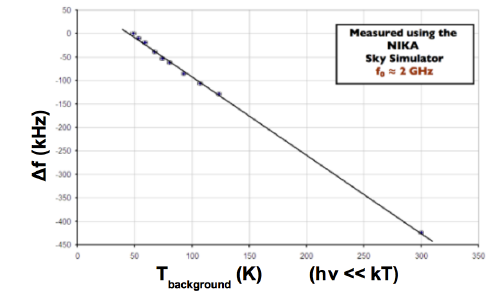
\includegraphics[scale=0.5]{Figures/KID-linearity-Monfardini2014.png}
	\caption{KID linarity demonstrated in laboratory under realistic conditions. Y-axis : frequency shift of the resonance (KID measured signal), X-axis : optical background temperature. The solid line represents the linear fit of the experimental points. Credits : \citet{2014JLTP..176..787M}.}
	\label{KID-lin}
\end{figure}

\begin{figure}[h]
	\includegraphics[scale=0.53]{Figures/epsilon.eps}
	\caption{KID non-linearity coefficient $\varepsilon$ as a function of number of points per $FWHM$. $\varepsilon$ was determined by using method 1 and method 2, for incoming fluxes between $1.10^{2}$ and $5.10^{4}$ AU.}
	\label{results_epsilon}
\end{figure}

Fig.\ref{results_epsilon} shows the non-linearity coefficient $\varepsilon$ derived, with the model described by Eq.\ref{fit_NL}, for different incoming flux. We can see that the non-linearity coefficients found by method 2 are lower than those found by method 1. Plus, the first method has shown that it is limited for incoming flux higher than $10^{4}$ as the signal is not perfectly reconstructed, whereas limite de la method 2.... To conclude, the second method is better than the first one which already reconstructed the signal very well.\\

Now that we have derived the non-linearity coefficient $\varepsilon$, we will see how to 


\subsection{Application to CMB maps and power spectra estimations}
The measurement of CMB polarization, and especially the detection of B modes, is one of the major challenges in modern cosmology. In this paper, we show that the KIDs systematic effect such as the non-linearity does not affect them from detecting B modes.

In this section we look at the next order correction, meaning that we will focus on the non-linear term produced by the detector and the way that we reconstruct the signal. A measure done by the KID is defined by $m = T + P$, with $T$ and $P$ representing the temperature and polarization. The non-linearity is characterized  by the $\varepsilon$ coefficient in $ m = m_{1} + \varepsilon m_{1}^{2}$. We have : 

\begin{equation}
\begin{split}
m & = m_{1} +\varepsilon' (T+P)^{2} \\
 & = T + P + \varepsilon'(T^{2} + P^{2} + 2TP) 
\end{split}
\end{equation}

Therefore, knowing that $T=I$ and $P = Q\cos(2\alpha) + U \sin(2\alpha)$, the polarized equation with a non-linear term is given Eq. \ref{eq-NL}.

\begin{equation}
m  \simeq (I + \varepsilon' I^{2}) + (Q + 2\varepsilon' IQ) \cos(2\alpha) + (U + 2 \varepsilon' IU) \sin(2\alpha)
\label{eq-NL}
\end{equation}

The non-linear coefficient $\varepsilon'$ is induced by the detector and the method used to reconstruct the signal.


The non-linearity coefficient $\varepsilon'$ does not intervene in the pointing strategy, in fact it is a systematic effect of the instrument and as a consequence will always impact our measurments. \\
To take into account this effect we simulate CMB maps with a PLANCK pointing strategy (citer ref) which follows Eq. \ref{eq-NL}, by using HEALPIX (citer ref).
Eq. \ref{eq-NL} is translated in the the power spectrum by Eq. \ref{eq-Cl}.

\begin{equation}
C_{l}^{s} \propto p^{2} \varepsilon^{2} C_{l}
\label{eq-Cl}
\end{equation}
Where $C_{l}^{s}$ is the systematic power spectra.\\

We generate I, Q, U maps from observed $C_{l}$ to which we apply the non-linear mapping described by Eq.\ref{eq-NL}. This will produce spurious polarization signals from which we can derive modified $C_{l}^{s}$ and $\varepsilon$ represented in Eq. \ref{eq-Cl}. We found 

\begin{equation}
\varepsilon^{2} \simeq 4.10^{-7}
\label{epsilon}
\end{equation}

This non-linearity can lead to leakage of the CMB temperature signal into the polarization maps and consequently can induce spurious polarization signals which could prevent us from detecting B mode polarization. The leakage effect is represented by the coefficient $\varepsilon$ of Eq. \ref{eq-Cl}. As a result, to be able to detect B mode polarization, the non-linearity coefficient related to the signal reconstruction must be lower than $\varepsilon^{2} \simeq 4.10^{-7}$.

%To do so, we calculate the non-linearity coefficient $\varepsilon'$ given by Eq.\ref{eq-NL} with a tolerance on mode B contamination by generating I, Q, U maps from observed $C_{l}$. Then we apply the non linear mapping described by Eq.\ref{eq-NL}, this will generate spurious signal from which we derive modified $C_{l}$. 


\subsection{Definition d'une strategie de pointage}

\subsection{HWP associated systematics}


\subsection{Cosmic rays impact on KIDs array}

One of the major problems for space based missions is the impact of an intense flux of high energy particles, referred to as Cosmic Rays (CR) on the detectors. Primary CR are produced by the Sun and by other galactic sources. They are mostly composed by protons (90\%), helium nuclei (9\%) and a few heavier nuclei and electrons (1\%). The CR spectrum is peaked aroud 200 MeV, thus the particles have sufficient energy to penetrate the detectors and give an unwanted signal. The Planck satellite \citep{2014A&A...571A..10P} has demonstrated that the impact of CR on the detectors are a key problem for space missions. Indeed, the glitches caused by CR can mask the real data and induce a loss of an important fraction of it.\\
Experiments have been done to construct a setup that allows to study the behavior of KIDs arrays under typical conditions of a space-borne observatory, and establish the compatibility of KIDs with a space environment \citep{2016A&A...592A..26C,2016SPIE.9914E..0NM}. When the detector is hit by a CR there is a lapse of time during which the sensor is 'blind' to the incoming scientific data. The length of this dead-time depends on the response time of the KID (time constant) which is determined by the quasi particle lifetime. \citet{2012ApPhL.100w2601M} have shown for KID, this time constant is equal to about tens of microseconds which is faster than bolometers (from 5-10 ms to 2s). This means that for the same CR hit, less data is lost when using KIDs arrays. Plus, the experiments have confirmed the fact that KID recover their initial state in less than 5 milliseconds. Finally, \citet{2016SPIE.9914E..0NM} concluded that the percent level of data loss per pixel by a KIDs array placed in a space environment is about 1 \% compared to 15 \% for Planck HFI bolometers.\\ The KID technology shows promising results for compatibility with a space-borne mission, as their extremely short glitch time constant permits to greatly reduce the data loss fraction due to CR impacts. 

